\documentclass[../../../../main.tex]{subfiles}

\begin{document}

\section*{第1問}

\noindent
[\textbf{解}] (イ) 判別式 $D$ として
\begin{align*}
D &= (a+c)^2 - 4(ac-b^2) \\
&= 4b^2 + (a-c)^2 \ge 0
\end{align*}
より、与方程式は実根を持つ。 \quad \text{同}

\vspace{0.5cm}

\noindent
(ロ)
\[
\begin{cases}
\alpha + \beta = a + c \\
\alpha \beta = ac - b^2
\end{cases}
\]
\[
\gamma - \alpha = \frac{a+c}{2} - \alpha - \frac{(a-c)(p^2-q^2)+4bpq}{2(p^2+q^2)}
\]
この正負は、以下とひとしい
\begin{align*}
A &= (a+c)(p^2+q^2) - 2\alpha(p^2+q^2) - (a-c)(p^2-q^2) - 4bpq \\
&= 2cp^2 + 2aq^2 - 2\alpha(p^2+q^2) - 4bpq
\end{align*}
\[
\frac{A}{2} = (c-\alpha)p^2 - 2bpq + (a-\alpha)q^2 \equiv f(p)
\]
$c = \alpha$ つまり $b=0$ の時、$f(p) = (a-\alpha)q^2 \ge 0$ となって $\gamma \ge \alpha$ である。 $c > \alpha$ の時、$f(p)=0$ の判別式 $D'$ として
\[
D'/4 = [b^2 - (c-\alpha)(a-\alpha)]q^2 = 0
\]
より、グラフの形を考えて $f(p) \ge 0 \iff \gamma \ge \alpha$。よっていずれの場合も $\gamma \ge \alpha \dots$ ①が成り立つ

\[
\beta - \gamma = \beta - \frac{a+c}{2} + \frac{(a-c)(p^2-q^2)+4bpq}{2(p^2+q^2)}
\]
この正負は、以下とひとしい
\begin{align*}
B &= 2\beta(p^2+q^2) - (a+c)(p^2+q^2) + (a-c)(p^2-q^2) + 4bpq \\
&= 2\beta(p^2+q^2) - 2aq^2 - 2cp^2 + 4bpq
\end{align*}
\[
\frac{B}{2} = (\beta-c)p^2 + 2bpq + (\beta-a)q^2 \equiv g(p)
\]
$\beta = c$ つまり $b=0$ のとき、$g(p) = (\beta-a)q^2 \ge 0$ から $\beta \ge \gamma$。 $\beta > c$ の時、同様に判別式 $D''$ として
\[
D''/4 = [b^2 - (\beta-c)(\beta-a)]q^2 = 0
\]
だから、$\beta \ge \gamma$。以上より $\beta \ge \gamma$ も成立つ $\dots$ ②

\noindent
①, ②から常に $\alpha \le \gamma \le \beta$ が成立する \quad \text{同}

\begin{center}
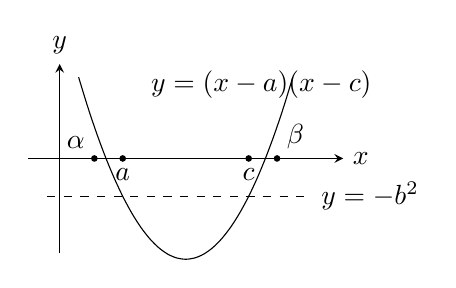
\begin{tikzpicture}[scale=0.8, >=stealth]
  \draw[->] (-0.5,0) -- (4.5,0) node[right] {$x$};
  \draw[->] (0,-1.5) -- (0,1.5) node[above] {$y$};
  \draw[domain=0.3:3.7, smooth, variable=\x] plot ({\x}, {(\x-1)*(\x-3)-0.6});
  \node[above] at (3.2,0.8) {$y=(x-a)(x-c)$};
  \draw[dashed] (-0.2,-0.6) -- (4.0,-0.6) node[right] {$y=-b^2$};
  \fill (0.55, 0) circle (1.5pt) node[above left] {$\alpha$};
  \fill (1, 0) circle (1.5pt) node[below] {$a$};
  \fill (3, 0) circle (1.5pt) node[below] {$c$};
  \fill (3.45, 0) circle (1.5pt) node[above right] {$\beta$};
\end{tikzpicture}
\end{center}
\noindent
※ 以上の証明に、$\alpha \le a, c \le \beta$ を用いたが、これはグラフより明らかである（対称性から $a \le c$ とした）

\newpage

\section*{第2問}

\noindent
[\textbf{解}] 内接円の半径 $r$, 外接円の半径 $R$ とおく。まず $\triangle ABC$ において内心 $O$ とし、図のように角度をおく ($\alpha+\beta+\gamma = \pi/2$) と
\[
AB = \frac{r}{\tan \alpha} + \frac{r}{\tan \beta}
\]
だから正弦定理から
\[
\frac{r}{\sin 2\gamma} \left( \frac{1}{\tan \alpha} + \frac{1}{\tan \beta} \right) = 2R
\]
$A = \sin \alpha \sin \beta \sin \gamma$ とおくと
\[
\frac{r \sin(\alpha+\beta)}{2A \cos \gamma} = 2R
\]
$\alpha+\beta+\gamma = \pi/2$ から $\sin(\alpha+\beta) = \sin(\pi/2-\gamma) = \cos \gamma$ だから
\[
A = \frac{r}{4R} \quad \dots \text{①}
\]
である。同様に $\triangle DEF$ において右のように角をおくと ($O''$ は $\triangle DEF$ の内心)
\[
\sin \alpha' \sin \beta' \sin \gamma' = \frac{r}{4R} \quad \dots \text{②}
\]
である。$\{\alpha, \beta, \gamma\} = \{\alpha', \beta', \gamma'\}$ ならば $\triangle ABC$ と $\triangle DEF$ は合同である $\dots$ ③。以下、
\begin{align*}
f(x, y) &= \sin x \sin y \sin(\pi/2 - x - y) \\
&= \sin x \sin y \cos(x+y) \quad (0 < x, y, \ x+y < \pi/2)
\end{align*}
のとりうる値を考える。もし、異なる2組の $(x,y)$ に対し $f(x,y)$ が同じ値をとるなら、①, ②から $\triangle ABC$ と $\triangle DEF$ は合同とは限らない $\dots$ ④

\[
f(x,y) = \frac{1}{2} \sin y \{ \sin(2x+y) - \sin y \}
\]
まず $y$ を固定して考える。$0 < x < \pi/2$ から $y < 2x+y < \pi-y$, $0 < y < \pi/2$ に注意して右辺 $g(y)$ とおくと
\[
0 < g(y) \le \frac{1}{2} \sin y (1 - \sin y) \quad \dots *
\]
次に $t = \sin y \ (0 < t < 1)$ とおいて、$y$ をうごかすことにより $S = g(y)$ のとりうる領域は下図斜線部である（境界は、斜線部のみ含む）。

\begin{center}
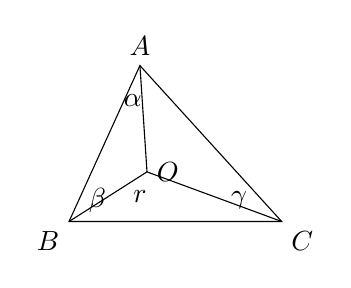
\begin{tikzpicture}[scale=0.9, >=stealth]
  \coordinate (A) at (1, 2.2);
  \coordinate (B) at (0, 0);
  \coordinate (C) at (3, 0);
  \coordinate (O) at (1.1, 0.7);
  
  \draw (A) -- (B) -- (C) -- cycle;
  \draw (A) -- (O);
  \draw (B) -- (O);
  \draw (C) -- (O);
  
  \node[above] at (A) {$A$};
  \node[below left] at (B) {$B$};
  \node[below right] at (C) {$C$};
  \node[right] at (O) {$O$};
  
  \node at (0.9, 1.7) {$\alpha$};
  \node at (0.4, 0.3) {$\beta$};
  \node at (2.4, 0.3) {$\gamma$};
  \node at (1.0, 0.35) {$r$};
\end{tikzpicture}
\hspace{0.5cm}
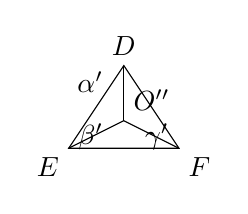
\begin{tikzpicture}[scale=0.7, >=stealth]
  \coordinate (D) at (1, 1.5);
  \coordinate (E) at (0, 0);
  \coordinate (F) at (2, 0);
  \coordinate (O2) at (1, 0.5);
  \draw (D) -- (E) -- (F) -- cycle;
  \draw (D) -- (O2);
  \draw (E) -- (O2);
  \draw (F) -- (O2);
  \node[above] at (D) {$D$};
  \node[below left] at (E) {$E$};
  \node[below right] at (F) {$F$};
  \node[left] at (0.8, 1.2) {$\alpha'$};
  \node at (0.4, 0.2) {$\beta'$};
  \node at (1.6, 0.2) {$\gamma'$};
  \node[above right] at (O2) {$O''$};
\end{tikzpicture}
\hspace{0.5cm}
\begin{tikzpicture}[scale=0.8, >=stealth]
  \draw[->] (-0.5,0) -- (3.0,0) node[right] {$t$};
  \draw[->] (0,-0.5) -- (0,2.0) node[above] {$S$};
  \node[below left] at (0,0) {$0$};
  
  \draw[domain=0:2.0, smooth, variable=\t, thick] plot ({\t}, {1.8*\t*(1-\t/2.0)});
  \fill[pattern=north east lines, pattern color=gray, domain=0:2.0, variable=\t] 
    plot ({\t}, {1.8*\t*(1-\t/2.0)}) -- (0,0) -- cycle;
    
  \draw[dashed] (1.0, 0) -- (1.0, 0.9) -- (0, 0.9);
  \node[below] at (1.0, 0) {$\frac{1}{2}$};
  \node[left] at (0, 0.9) {$\frac{1}{8}$};
  \node[below] at (2.0, 0) {$1$};
\end{tikzpicture}
\end{center}

\noindent
今、①, ②を満たす文字の存在は保障されていることから③, ④より
\[
0 < \frac{r}{4R} < \frac{1}{8} \text{ の時、合同とは限らない}
\]
\[
\frac{r}{4R} = \frac{1}{8} \text{ の時、合同}
\]
($\because 0 < y < \pi/2$ から $t = 1/2 \iff y = \pi/6$, で、等号が成立することから $2x+\pi/6 = \pi/2 \iff x = \pi/6$)

\newpage

\section*{第3問}

\noindent
[\textbf{解}] 答案を書き直し、修正部分には \underline{\hspace{0.8cm}} を下に引く。

\vspace{0.3cm}

\noindent
$(1)\times y - (2)\times x \implies (y-\underline{x})z(z+1)=0$

\noindent
から (イ) $z=0$, (ロ) $z=-1$, (ハ) $y=x$

\vspace{0.3cm}

\noindent
(イ)の時、(1),(2),(3)から $(x,y,z)=(0,0,0)$

\noindent
(ロ)の時、(1),(2)から $x=y=0$ だが、これは \underline{(3)を満たさず不適}

\noindent
(ハ)の時、(3)から $z^2(z+y+2)=0$, (イ)で $z=0$ は考えたので $z \neq 0$ として $z+y+2=0 \iff z=-(y+2)$ だから (2)に代入
\[
-y(y+2) = y + (y+2)^2 - (y+2)
\]
\[
y^2 + 3y + 1 = 0
\]
\[
y = \frac{-3 \mp \sqrt{5}}{2}
\]
$z=-(y+2)$ に代入して
\[
z = - \underline{\frac{1 \mp \sqrt{5}}{2} = \frac{-1 \pm \sqrt{5}}{2}}
\]
だから, $x = \frac{-3 \mp \sqrt{5}}{2}$

\vspace{0.3cm}

\noindent
以上から
\[
(x,y,z) = (0,0,0), \ \underline{\left( \frac{-3 \mp \sqrt{5}}{2}, \frac{-3 \mp \sqrt{5}}{2}, \frac{-1 \pm \sqrt{5}}{2} \right)}
\]

\newpage

\section*{第4問}

\noindent
[\textbf{解}] (イ) $A(0,a), B(b,0), C(-c,0) \ (a,b,c > 0)$ とおく。 $D,E,F$ の時刻 $t$ での座標は題意より
\begin{align*}
\vec{OD} &= \begin{pmatrix} 0 \\ a \end{pmatrix} + t \begin{pmatrix} b \\ -a \end{pmatrix} \\
\vec{OE} &= \begin{pmatrix} b \\ 0 \end{pmatrix} + t \begin{pmatrix} -c-b \\ 0 \end{pmatrix} \quad \dots \text{①} \\
\vec{OF} &= \begin{pmatrix} -c \\ 0 \end{pmatrix} + t \begin{pmatrix} c \\ a \end{pmatrix}
\end{align*}
だから、$\triangle DEF$ の重心 $G(X,Y)$ とすると
\begin{align*}
X &= \frac{1}{3} [ tb + b + t(-c-b) - c + tc ] = \frac{1}{3} (b-c) \\
Y &= \frac{1}{3} [ a - ta + ta ] = \frac{1}{3} a
\end{align*}
となって、はじめの重心からうごかない \quad \text{同}

\vspace{0.5cm}

\noindent
(ロ) ①から
\begin{align*}
\vec{ED} &= \begin{pmatrix} tb \\ a(1-t) \end{pmatrix} - \begin{pmatrix} b-t(b+c) \\ 0 \end{pmatrix} = \begin{pmatrix} -b+t(2b+c) \\ a(1-t) \end{pmatrix} \\
\vec{EF} &= \begin{pmatrix} c(t-1) \\ ta \end{pmatrix} - \begin{pmatrix} b-t(b+c) \\ 0 \end{pmatrix} = \begin{pmatrix} -b-c+t(b+2c) \\ ta \end{pmatrix}
\end{align*}
だから、時刻 $t$ での $\triangle DEF$ の面積 $S(t)$ は
\begin{align*}
S(t) &= \frac{1}{2} \left| [-b+t(2b+c)] ta - [-b-c+t(b+2c)] a(1-t) \right| \\
&= \frac{1}{2} a \left| -bt + (2b+c)t^2 + (b+2c)t^2 - (2b+3c)t + b+c \right| \\
&= \frac{1}{2} a \left| 3(b+c)t^2 - 3(b+c)t + b+c \right| \\
&= \frac{1}{2} a(b+c) \left| 3t^2 - 3t + 1 \right| \\
&= \frac{1}{2} a(b+c) \left| 3\left(t - \frac{1}{2}\right)^2 + \frac{1}{4} \right|
\end{align*}
より、$S(t)$ は $t = 1/2$ の時 min で、この時 $\triangle ABC$ の面積 $S$ として
\[
\frac{S(1/2)}{S} = \frac{1}{4} \text{ 倍である。}
\]

\newpage

\section*{第5問}

\noindent
[\textbf{解}] $\triangle O P_n P_{n+1}$ と $\triangle O P_{n+1} P_{n+2}$ の相似比は、
\[
\frac{|O P_{n+1}|}{|O P_n|} \text{ である。} \quad \dots \text{①}
\]
ここで $\triangle O P_0 P_1$ に正弦定理を用いて、
\[
\frac{|O P_1|}{\sin \theta} = \frac{\alpha}{\sin(\alpha+\theta)} \implies |O P_1| = \frac{\sin \theta}{\sin(\alpha+\theta)} \cdot \alpha \quad \dots \text{②}
\]
だから、$\alpha \neq 0$ より、①から
\[
\frac{|O P_1|}{|O P_0|} = 1 \cdot \frac{\sin \theta}{\sin(\alpha+\theta)}
\]
したがって、$0 < \frac{\sin \theta}{\sin(\alpha+\theta)} < 1$ ならば $P_n$ は $O$ に収束する。 （以上 (イ)）

\begin{center}
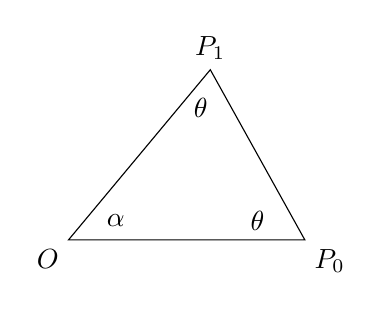
\begin{tikzpicture}[scale=1.2, >=stealth]
  \coordinate (O) at (0,0);
  \coordinate (P0) at (2.5,0);
  \coordinate (P1) at (1.5, 1.8);
  \draw (O) -- (P0) -- (P1) -- cycle;
  \node[below left] at (O) {$O$};
  \node[below right] at (P0) {$P_0$};
  \node[above] at (P1) {$P_1$};
  \node at (0.5, 0.2) {$\alpha$};
  \node at (2.0, 0.2) {$\theta$};
  \node at (1.4, 1.4) {$\theta$};
\end{tikzpicture}
\end{center}

\noindent
さて、$\triangle O P_n P_{n+1}$ の面積 $S_n$ とする。まず、
\[
S_0 = \frac{1}{2} |O P_0| |O P_1| = \frac{1}{2} \cdot \frac{\sin \theta}{\sin(\alpha+\theta)} \alpha^2 \quad \dots \text{③}
\]
であり、①から、$p = \frac{\sin \theta}{\sin(\alpha+\theta)}$ として
\[
S_{n+1} = p^2 S_n
\]
くり返し用いて、③から
\[
S_n = (p^2)^{n-1} \cdot \frac{1}{2} p \alpha^2 = \frac{1}{2} p^{2n-1} \alpha^2
\]
したがって、$0 < p < 1$ とあわせて、
\[
S = \lim_{n \to \infty} \sum_{k=0}^n S_k = \frac{1}{2} p \alpha^2 \frac{1}{1-p^2}
\]
だから、$S$ は $\triangle O P_0 P_1$ の
\[
\frac{1}{1-p^2} = \frac{1}{1 - \left( \frac{\sin \theta}{\sin(\alpha+\theta)} \right)^2} \text{ (倍)}
\]
である。(以上 (ロ))

\vspace{0.5cm}

\noindent
ここで、$a_n = |P_n P_{n+1}|$ とおく。①から
\[
a_{n+1} = p a_n \quad \dots \text{④}
\]
であり、$\triangle O P_0 P_1$ に正弦定理を用いて、
\[
\frac{|P_0 P_1|}{\sin \theta} = \frac{\alpha}{\sin(\alpha+\theta)} \implies a_0 = \frac{\sin \theta}{\sin(\alpha+\theta)} \alpha
\]
だから、④をくり返し用いて、
\[
a_n = \frac{\sin \theta}{\sin(\alpha+\theta)} \alpha \cdot p^{n-1}
\]
となるので、
\begin{align*}
L &= \lim_{n \to \infty} \sum_{k=0}^n a_k = \frac{\sin \theta \cdot \alpha}{\sin(\alpha+\theta)} \cdot \frac{1}{1-p} \quad (\because |p| < 1) \\
&= \frac{\sin \theta \cdot \alpha}{\sin(\alpha+\theta)} \cdot \frac{\sin(\alpha+\theta)}{\sin(\alpha+\theta) - \sin \theta} = \frac{\sin \theta}{\sin(\alpha+\theta) - \sin \theta} \cdot \alpha
\end{align*}
である。$\theta \to +0$ として、
\[
L = \frac{\theta}{\sin(\alpha+\theta) - \sin \theta} \cdot \frac{\sin \theta}{\theta} \cdot \alpha \longrightarrow \frac{\alpha}{\cos \alpha}
\]

\newpage

\section*{第6問}

\noindent
[\textbf{解}] $f(x) = \int_0^x \cos t \, dt - 2 \int_0^x \sin t \, dt$ とおく。

\noindent
$f'(x) = \cos x - 2 \sin x$ で、これは区間 $[0, \pi/4]$ で単調減少かつ、$f'(\pi/6) = 0$ より、下表を与える

\begin{center}
\begin{tabular}{c|ccccc}
$x$ & $0$ & $\dots$ & $\pi/6$ & $\dots$ & $\pi/4$ \\ \hline
$f'$ & & $+$ & $0$ & $-$ & \\ \hline
$f$ & & $\nearrow$ & & $\searrow$ &
\end{tabular}
\end{center}

\noindent
これより、$f(0)=0$, $f(\pi/4) = [\sin t + 2 \cos t]_0^{\pi/4} = \frac{3}{\sqrt{2}} - 2 > 0$ から、$f(x) > 0 \ (0 < x < \pi/4)$ なので、題意は示された \quad \text{同}

\end{document}
